\chapter{Specifikacija programske potpore}
		
	\section{Funkcionalni zahtjevi}
					
			\noindent \textbf{Dionici:}
			
			\begin{packed_enum}
				
				\item Administrator
				\item Organizatori događaja
				\item Građani (posjetitelji)
				\item Razvojni tim				
				
			\end{packed_enum}
			
			\noindent \textbf{Aktori i njihovi funkcionalni zahtjevi:}
			
			
			\begin{packed_enum}
				\item  \underbar{Neregistrirani/neprijavljeni korisnik (inicijator) može:}
				
				\begin{packed_enum}
					
					\item stvoriti novi korisnički račun kao:
					\begin{packed_enum}
						\item organizator (naziv, e-mail adresa, lozinka, adresa, poveznica na vlastite web ili Facebook stranice) 
						\item  posjetitelj (ime, prezime, korisničko ime, e-mail adresa, lozinka) 
					\end{packed_enum} 
					\item prijaviti se u sustav
					
				\end{packed_enum}
			
				\item  \underbar{Posjetitelj (inicijator) može:}
				
				\begin{packed_enum}
					
					\item prijaviti se u sustav i odjaviti iz sustava
					\item pregledavati i uređivati svoje osobne podatke
					\item vidjeti popis aktualnih događanja u odabranom vremenskom razdoblju (24 sata, 7 dana, 30 dana)
					\item odabrati postavke da im aplikacija automatski šalje obavijesti o najnovijim događanjima (prema vrsti događanja i području) 
					\item za svako događanje: 
					\begin{packed_enum}
						\item iskazati interes (\textit{sigurno dolazim, možda dolazim, ne dolazim})
						\item po želji promijeniti interes
					\end{packed_enum} 
					\item vidjeti podatke o organizatorima događanja (naziv, adresa, poveznica na vlastite web ili Facebook stranice,  popis svih događanja koja su oglašena putem aplikacije u zadnje 2 godine)
					\item napisati recenziju (i/ili obrisati svoju napisanu recenziju) za događanja koja su završila u posljednjih 48 sati
					\item obrisati svoj korisnički račun
					\item odjaviti se iz sustava
					
				\end{packed_enum}
		
				\item \underbar{Organizator (inicijator) može:}		
						
				\begin{packed_enum}
					\item sve što može i Posjetitelj
					\item stvoriti novo događanje:
					\begin{packed_enum}
						\item za koje se ne plaća ulaz (*navesti podatke*)
						\item za koje se plaća ulaz ()
					\end{packed_enum}
					\item pregledavati i brisati svoja događanja 
				\end{packed_enum}
				
				\item \underbar{Administrator (inicijator) može:}
				
				\begin{packed_enum}
					\item prijaviti se u sustav
					\item vidjeti popis i osobne podatke svih registriranih korisnika 
					\item trajno obrisati korisnički profil
					\item postaviti cijenu članarine za organizatore događanja za koje se plaća ulaz
					\item brisati recenzije i događanja 
					\item odjaviti se iz sustava
				\end{packed_enum}
				
				\item \underbar{Baza podataka (sudionik):}
				\begin{packed_enum}
					\item pohranjuje podatke registriranih korisnika 
					\item pohranjuje podatke o događanjima 
					\item pohranjuje recenzije događanja 
				\end{packed_enum}
			\end{packed_enum}
			
			\eject 
			
			
				
			\subsection{Obrasci uporabe}
				
				\subsubsection{Opis obrazaca uporabe}
						

					\noindent \underbar{\textbf{UC1 - Registracija}}
					\begin{packed_item}
	
						\item \textbf{Glavni sudionik:} Neregistrirani/neprijavljeni korisnik
						\item  \textbf{Cilj:} Stvaranje korisničkog računa za korištenje platforme
						\item  \textbf{Sudionici:} Baza podataka
						\item  \textbf{Preduvjet:} -
						\item  \textbf{Opis osnovnog tijeka:}
						
						\item[] \begin{packed_enum}
	
							\item Korisnik odabire opciju registracije
							\item Korisnik unosi tražene podatke
							\item Korisnik dobiva pristup korisničkim funkcijama i obavijest o uspješnoj registraciji te se preusmjerava na početnu stranicu za prijavljene korisnike 
							
						\end{packed_enum}
						
						\item  \textbf{Opis mogućih odstupanja:}
						
						\item[] \begin{packed_item}
							
							\item[2.a] Uneseno zauzeto korisničko ime i/ili e-mail adresa, korisničko ime i/ili lozinka u nedozvoljenom formatu, neispravna e-mail adresa 
							\item[] \begin{packed_enum}
								
								\item Obavijestiti korisnika o neispravnom unosu i omogućiti ponovni unos neprihvaćenih vrijednosti
								\item Korisnik unosi nove vrijednosti i uspješno završava registraciju ili odustaje od registracije 
								
							\end{packed_enum}
						\end{packed_item}
					
					\end{packed_item}
					
%	%	%	%	%	%	%	%	%	%	%	%	%	%	%	%	%	%	%
					
					\noindent \underbar{\textbf{UC2 - Prijava}}
					\begin{packed_item}
						
						\item \textbf{Glavni sudionik:} Neregistrirani/neprijavljeni korisnik
						\item  \textbf{Cilj:} Dobiti pristup odgovarajućem korisničkom sučelju ovisno o ulozi 
						\item  \textbf{Sudionici:} Baza podataka
						\item  \textbf{Preduvjet:} Registracija
						\item  \textbf{Opis osnovnog tijeka:}
						
						\item[] \begin{packed_enum}
							
							\item Korisnik odabire opciju prijave u sustav
							\item Korisnik unosi tražene podatke (korisničko ime i lozinka)
							\item Provjera ispravnosti unesenih podataka 
							\item Korisnik dobiva obavijest o uspješnoj prijavi i preusmjerava se na početnu stranicu za prijavljene korisnike 
							
						\end{packed_enum}
						
						\item  \textbf{Opis mogućih odstupanja:}
						
						\item[] \begin{packed_item}
							
							\item[2.a] Uneseno neispravno korisničko ime i/ili lozinka  
							\item[] \begin{packed_enum}
								
								\item Obavijestiti korisnika o neuspješnoj registraciji i omogućiti ponovni unos korisničkog imena i/ili lozinke
								\item Korisnik unosi nove vrijednosti i uspješno se prijavljuje ili odustaje od prijave
								
							\end{packed_enum}
						\end{packed_item}
						
					\end{packed_item}
					
%	%	%	%	%	%	%	%	%	%	%	%	%	%	%	%	%	%	%
					
					
					\noindent \underbar{\textbf{UC3 - Odjava}}
					\begin{packed_item}
						
						\item \textbf{Glavni sudionik:} Prijavljeni korisnik (Administrator, Organizator, Posjetitelj)
						\item  \textbf{Cilj:} Odjava iz sustava 
						\item  \textbf{Sudionici:} Baza podataka
						\item  \textbf{Preduvjet:} Korisnik je trenutno prijavljen u sustav
						\item  \textbf{Opis osnovnog tijeka:}
						
						\item[] \begin{packed_enum}
							
							\item Korisnik odabire opciju odjave
							\item Korisnik gubi pristup korisničkim funkcijama
							\item Korisnik se preusmjerava na početnu stranicu za neregistrirane/neprijavljene korisnike 
							
						\end{packed_enum}
					\end{packed_item}
					
%	%	%	%	%	%	%	%	%	%	%	%	%	%	%	%	%	%	%
					
					\noindent \underbar{\textbf{UC4 - Pregled osobnih podataka}}
					\begin{packed_item}
						
						\item \textbf{Glavni sudionik:} Korisnik (Organizator, Posjetitelj)
						\item  \textbf{Cilj:} Pregledati osobne podatke
						\item  \textbf{Sudionici:} Baza podataka
						\item  \textbf{Preduvjet:} Korisnik je trenutno prijavljen u sustav
						\item  \textbf{Opis osnovnog tijeka:}
						
						\item[] \begin{packed_enum}
							
							\item Korisnik odabire opciju za pregled svog profila
							\item Prikazuju se osobni podaci vezani uz korisnički račun
					 
						\end{packed_enum}
					\end{packed_item}
					
%	%	%	%	%	%	%	%	%	%	%	%	%	%	%	%	%	%	%
					
					\noindent \underbar{\textbf{UC5 - Uređivanje osobnih podataka}}
					\begin{packed_item}
						
						\item \textbf{Glavni sudionik:} Korisnik (Organizator, Posjetitelj)
						\item  \textbf{Cilj:} Izmijeniti osobne podatke 
						\item  \textbf{Sudionici:} Baza podataka
						\item  \textbf{Preduvjet:} Korisnik je trenutno prijavljen u sustav
						\item  \textbf{Opis osnovnog tijeka:}
						
						\item[] \begin{packed_enum}
							
							\item Korisnik odabire opciju izmjene osobnih podataka
							\item Korisnik mijenja željene podatke 
							\item Provjera ispravnosti unesenih podataka 
							\item Korisnik sprema promjene
							\item Baza podataka se osvježava 
							
						\end{packed_enum}
						
						\item  \textbf{Opis mogućih odstupanja:}
						
						\item[] \begin{packed_item}
							
							\item[2.a] Novo uneseni podaci su nedozvoljene vrijednosti
							\item[] \begin{packed_enum}
								
								\item Onemogućiti spremanje promjena
								\item Obavijestiti korisnika o nedozvoljenim vrijednostima i omogućiti ponovni unos 
								\item Korisnik unosi nove vrijednosti i omogućava se spremanje promjena
								
							\end{packed_enum}
							
							\item[4.a] Korisnik pokušava napustiti prozor, a nije spremio promjene 
							\item[] \begin{packed_enum}
								
								\item Obavijestiti korisnika o obaveznom spremanju promjena
								\item Nakon spremanja promjena omogućiti izlaz iz prozora
								
							\end{packed_enum}
							
						\end{packed_item}
						
					\end{packed_item}
					
%	%	%	%	%	%	%	%	%	%	%	%	%	%	%	%	%	%	%
					
					\noindent \underbar{\textbf{UC6 - Postavke obavještavanja o novim događanjima}}
					\begin{packed_item}
						
						\item \textbf{Glavni sudionik:} Prijavljeni korisnik (Organizator, Posjetitelj)
						\item  \textbf{Cilj:} Podesiti postavke obavještavanja o najnovijim događanjima
						\item  \textbf{Sudionici:} Baza podataka
						\item  \textbf{Preduvjet:} Korisnik je trenutno prijavljen u sustav i ima ovlasti Posjetitelja
						\item  \textbf{Opis osnovnog tijeka:}
						
						\item[] \begin{packed_enum}
							
							\item Korisnik odabire opciju uređivanja postavki obavještavanja o novim događanjima
							\item Korisnik odabire želi li primati obavijesti i, ako da, o kojim vrstama događanja i iz kojeg područja
							\item Korisnik sprema promjene
							\item Baza podataka se osvježava
							
						\end{packed_enum}
						
						\item  \textbf{Opis mogućih odstupanja:}
						
						\item[] \begin{packed_item}
							
							\item[2.a] Korisnik odabire da želi primati obavijesti, ali ne unese minimalno jednu vrstu događanja i minimalno jedno područje
							\item[] \begin{packed_enum}
								
								\item Onemogućiti spremanje promjena
								\item Obavijestiti korisnika o obaveznom izboru barem jedne vrste događanja i barem jednog područja
								\item Korisnik odabire vrstu događanja i/ili područje koje nedostaje i omogućava se spremanje promjena
								
							\end{packed_enum}
						\end{packed_item}
						
					\end{packed_item}
					
%	%	%	%	%	%	%	%	%	%	%	%	%	%	%	%	%	%	%

					\noindent \underbar{\textbf{UC7 - Brisanje vlastitog korisničkog računa}}
					\begin{packed_item}
						
						\item \textbf{Glavni sudionik:} Korisnik (Organizator, Posjetitelj)
						\item  \textbf{Cilj:} Obrisati korisnički račun i sve osobne podatke
						\item  \textbf{Sudionici:} Baza podataka
						\item  \textbf{Preduvjet:} Korisnik je trenutno prijavljen u sustav
						\item  \textbf{Opis osnovnog tijeka:}
						
						\item[] \begin{packed_enum}
							
							\item Korisnik odabire opciju brisanja korisničkog računa
							\item Korisnik potvrđuje svoj odabir 
							\item Baza podataka se osvježava
							\item Korisnik se preusmjerava na početnu stranicu za neregistrirane/neprijavljene korisnike 
							
						\end{packed_enum}
						
					\end{packed_item}
					
%	%	%	%	%	%	%	%	%	%	%	%	%	%	%	%	%	%	%

					\noindent \underbar{\textbf{UC8 - Pregled svih korisničkih računa}}
					\begin{packed_item}
						
						\item \textbf{Glavni sudionik:} Administrator
						\item  \textbf{Cilj:} Prikaz svih korisničkih računa 
						\item  \textbf{Sudionici:} Baza podataka
						\item  \textbf{Preduvjet:} Korisnik je trenutno prijavljen u sustav i ima ovlasti Administratora
						\item  \textbf{Opis osnovnog tijeka:}
						
						\item[] \begin{packed_enum}
							
							\item Administrator odabire opciju pregleda korisničkih računa
							\item Prikazuje se popis svih korisničkih računa
							
						\end{packed_enum}
						
					\end{packed_item}
					
%	%	%	%	%	%	%	%	%	%	%	%	%	%	%	%	%	%	%
					
					\noindent \underbar{\textbf{UC9 - Brisanje korisničkog računa}}
					\begin{packed_item}
						
						\item \textbf{Glavni sudionik:} Administrator
						\item  \textbf{Cilj:} Trajno brisanje korisnika iz sustava
						\item  \textbf{Sudionici:} Baza podataka
						\item  \textbf{Preduvjet:} Korisnik je prijavljen, ima ovlasti Administratora i prikazan mu je popis svih korisničkih računa
						\item  \textbf{Opis osnovnog tijeka:}
						
						\item[] \begin{packed_enum}
							
							\item Administrator odabire opciju brisanja korisničkog računa 
							\item Administrator potvrđuje svoj odabir
							\item Baza podataka se osvježava
							\item Promjena je vidljiva u prikazanom popisu korisničkih računa
							
						\end{packed_enum}
						
					\end{packed_item}
					
%	%	%	%	%	%	%	%	%	%	%	%	%	%	%	%	%	%	%
					
						\noindent \underbar{\textbf{UC10 - Postavljanje cijene članarine}}
					\begin{packed_item}
						
						\item \textbf{Glavni sudionik:} Administrator
						\item  \textbf{Cilj:} Postavljanje cijene mjesečne članarine za organizatore
						\item  \textbf{Sudionici:} Baza podataka
						\item  \textbf{Preduvjet:} Korisnik je prijavljen i ima ovlasti Administratora 
						\item  \textbf{Opis osnovnog tijeka:}
						
						\item[] \begin{packed_enum}
							
							\item Administrator odabire opciju postavljanja članarine
							\item Administrator unosi cijenu i sprema ju
							\item Baza podataka se osvježava
							
						\end{packed_enum}
						
						\item  \textbf{Opis mogućih odstupanja:}
						
						\item[] \begin{packed_item}
							
							\item[2.a] Unesena cijena nije ispravnog formata
							\item[] \begin{packed_enum}
								
								\item Onemogućiti spremanje promjena
								\item Obavijestiti korisnika o nedozvoljenoj vrijednosti i omogućiti ponovni unos 
								\item Korisnik unosi novu vrijednost i omogućava se spremanje promjena
								
							\end{packed_enum}
						\end{packed_item}
						
					\end{packed_item}
					
%	%	%	%	%	%	%	%	%	%	%	%	%	%	%	%	%	%	%

					\noindent \underbar{\textbf{UC11 - Dodavanje novog događanja}}
					\begin{packed_item}
						
						\item \textbf{Glavni sudionik:} Organizator
						\item  \textbf{Cilj:} Dodati novo događanje 
						\item  \textbf{Sudionici:} Baza podataka
						\item  \textbf{Preduvjet:} Korisnik je prijavljen i ima ovlasti Organizatora
						\item  \textbf{Opis osnovnog tijeka:}
						
						\item[] \begin{packed_enum}
							
							\item Organizator odabire opciju dodavanja novog događanja
							\item Organizator upisuje potrebne i, po želji, opcionalne podatke o događanju (naziv, vrsta, lokacija, vrijeme početka, trajanje, cijena; opcionalno foto/video galerija)
							\item Organizator odabire plaća li se događanje (određuje cijenu ili naglašava da je besplatno):
							
							\item[] \begin{packed_enum}
								
								\item ako se događanje plaća i organizator još nema plaćenu članarinu, prije objave događanja mora podmiriti članarinu 
								\item ako se događanje ne plaća ili se događanje plaća i članarina je podmirena, može samo nastaviti objavu događanja
								
							\end{packed_enum}
							
							\item Organizator dovršava objavu i objavljuje ju
							\item Baza podataka se osvježava
							\item Događanje će biti prikazano na stranici
							
							\end{packed_enum}
							
							\item  \textbf{Opis mogućih odstupanja:}
							
							\item[] \begin{packed_item}
								
								\item[2.a] Uneseni podaci su nedozvoljene vrijednosti
								\item[] \begin{packed_enum}
									
									\item Onemogućiti završetak dodavanja događanja
									\item Obavijestiti korisnika o nedozvoljenim vrijednostima i omogućiti ponovni unos 
									\item Korisnik unosi nove vrijednosti i omogućava se nastavak na objavu događanja
									
								\end{packed_enum}		
							\end{packed_item}
							
					\end{packed_item}
					
%	%	%	%	%	%	%	%	%	%	%	%	%	%	%	%	%	%	%
					\newpage

					\noindent \underbar{\textbf{UC12 - Pregled svih događanja}}
					\begin{packed_item}
						
						\item \textbf{Glavni sudionik:} Prijavljeni korisnik (Posjetitelj, Organizator, Administrator)
						\item  \textbf{Cilj:} Pregled svih događanja prema određenom kriteriju
						\item  \textbf{Sudionici:} Baza podataka
						\item  \textbf{Preduvjet:} Korisnik je trenutno prijavljen u sustav 
						\item  \textbf{Opis osnovnog tijeka:}
						
						\item[] \begin{packed_enum}
							
							\item Na početnoj stranici korisnik odabire kriterij prema kojem se prikazuju događanja (prikaz događanja završenih u zadnjih 48 sati ili aktualna događanja u narednih 24 sata, 7 dana, 30 dana)
							\item Događanja koja zadovoljavaju odabrani kriterij prikazuju se na stranici
						
						\end{packed_enum}
						
					\end{packed_item}
					
%	%	%	%	%	%	%	%	%	%	%	%	%	%	%	%	%	%	%

					\noindent \underbar{\textbf{UC13 - Pregled jednog događanja}}
					\begin{packed_item}
						
						\item \textbf{Glavni sudionik:} Prijavljeni korisnik (Posjetitelj, Organizator, Administrator)
						\item  \textbf{Cilj:} Pregled jednog odabranog događanja od svih prikazanih događanja
						\item  \textbf{Sudionici:} Baza podataka
						\item  \textbf{Preduvjet:} Korisnik je trenutno prijavljen u sustav i prikazana su sva događanja prema odabranom kriteriju
						\item  \textbf{Opis osnovnog tijeka:}
						
						\item[] \begin{packed_enum}
							
							\item Korisnik odabire jedno od prikazanih događanja
							\item Na zasebnoj se stranici korisniku prikazuju detalji o odabranom događanju
							
						\end{packed_enum}
						
					\end{packed_item}
					
%	%	%	%	%	%	%	%	%	%	%	%	%	%	%	%	%	%	%				
					
					\noindent \underbar{\textbf{UC14 - Pregled profila organizatora}}
					\begin{packed_item}
						
						\item \textbf{Glavni sudionik:} Prijavljeni korisnik (Posjetitelj, Organizator)
						\item  \textbf{Cilj:} Pregled korisničkog računa organizatora
						\item  \textbf{Sudionici:} Baza podataka
						\item  \textbf{Preduvjet:} Korisnik je trenutno prijavljen u sustav, ima ovlasti Posjetitelja ili Organizatora i ima otvoren prikaz nekog događanja
						\item  \textbf{Opis osnovnog tijeka:}
						
						\item[] \begin{packed_enum}
							
							\item Posjetitelj odabire opciju prikaza profila organizatora
							\item Prikazuju se informacije o organizatoru
							
						\end{packed_enum}
						
					\end{packed_item}
					
%	%	%	%	%	%	%	%	%	%	%	%	%	%	%	%	%	%	%
					\newpage
					
					\noindent \underbar{\textbf{UC15 - Pregled vlastitih događanja}}
					\begin{packed_item}
						
						\item \textbf{Glavni sudionik:} Organizator
						\item  \textbf{Cilj:} Pregled svih događanja koje je taj organizator objavio
						\item  \textbf{Sudionici:} Baza podataka
						\item  \textbf{Preduvjet:} Korisnik je trenutno prijavljen u sustav i ima ovlasti Organizatora  
						\item  \textbf{Opis osnovnog tijeka:}
						
						\item[] \begin{packed_enum}
							
							\item Organizator odabire opciju prikaza vlastitih događanja
							\item Ovisno o tome ima li organizator objavljenih događanja prikazuju se događanja ili odgovarajuća poruka
							
						\end{packed_enum}
						
					\end{packed_item}
					
%	%	%	%	%	%	%	%	%	%	%	%	%	%	%	%	%	%	%
					
					\noindent \underbar{\textbf{UC16 - Pregled jednog vlastitog događanja}}
					\begin{packed_item}
						
						\item \textbf{Glavni sudionik:} Organizator
						\item  \textbf{Cilj:} Prikaz jednog od događanja koje je taj organizator objavio
						\item  \textbf{Sudionici:} Baza podataka
						\item  \textbf{Preduvjet:} Korisnik je trenutno prijavljen u sustav, ima ovlasti Organizatora i prikazana su mu sva vlastita događanja
						\item  \textbf{Opis osnovnog tijeka:}
						
						\item[] \begin{packed_enum}
							
							\item Organizator odabire opciju prikaza jednog od događanja
							\item Na zasebnoj se stranici organizatoru prikazuju detalji o odabranom događaju (uključujući i recenzije posjetitelja)
							
						\end{packed_enum}
						
					\end{packed_item}
					
%	%	%	%	%	%	%	%	%	%	%	%	%	%	%	%	%	%	%

					\noindent \underbar{\textbf{UC17 - Brisanje vlastitog događanja}}
					\begin{packed_item}
						
						\item \textbf{Glavni sudionik:} Organizator
						\item  \textbf{Cilj:} Trajno brisanje vlastitog događanja
						\item  \textbf{Sudionici:} Baza podataka
						\item  \textbf{Preduvjet:} Korisnik je prijavljen, ima ovlasti Organizatora i prikazana su mu sva vlastita događanja
						\item  \textbf{Opis osnovnog tijeka:}
						
						\item[] \begin{packed_enum}
							
							\item Organizator odabire opciju brisanja događanja
							\item Organizator potvrđuje svoj odabir
							\item Baza podataka se osvježava
							\item Promjena je vidljiva u prikazanom popisu događanja
							
						\end{packed_enum}
						
					\end{packed_item}
					
%	%	%	%	%	%	%	%	%	%	%	%	%	%	%	%	%	%	%
					\newpage
										
					\noindent \underbar{\textbf{UC18 - Brisanje događanja}}
					\begin{packed_item}
						
						\item \textbf{Glavni sudionik:} Administrator
						\item  \textbf{Cilj:} Trajno brisanje događanja
						\item  \textbf{Sudionici:} Baza podataka
						\item  \textbf{Preduvjet:} Korisnik je prijavljen, ima ovlasti Administratora i prikazana su mu sva događanja
						\item  \textbf{Opis osnovnog tijeka:}
						
						\item[] \begin{packed_enum}
							
							\item Administrator odabire opciju brisanja događanja
							\item Administrator potvrđuje svoj odabir
							\item Baza podataka se osvježava
							\item Promjena je vidljiva u prikazanom popisu događanja
							
						\end{packed_enum}
						
					\end{packed_item}
					
%	%	%	%	%	%	%	%	%	%	%	%	%	%	%	%	%	%	%

					\noindent \underbar{\textbf{UC19 - Recenziranje događanja}}
					\begin{packed_item}
						
						\item \textbf{Glavni sudionik:} Prijavljeni korisnik (Organizator, Posjetitelj)
						\item  \textbf{Cilj:} Dodavanje recenzije događanja
						\item  \textbf{Sudionici:} Baza podataka
						\item  \textbf{Preduvjet:} Korisnik je prijavljen, ima ovlasti Posjetitelja ili Organizatora i otvoren je prikaz događanja koje je završilo u posljednjih 48 sati
						\item  \textbf{Opis osnovnog tijeka:}
						
						\item[] \begin{packed_enum}
							
							\item Posjetitelj odabire opciju dodavanja recenzije
							\item Posjetitelj upisuje recenziju
							\item Posjetitelj potvrđuje da želi objaviti recenziju ili odustaje od objave
							\item Baza podataka se osvježava
							\item Recenzija je dodana i vidljiva na vrhu recenzija tog događanja

						\end{packed_enum}
						
						\item  \textbf{Opis mogućih odstupanja:}
						
						\item[] \begin{packed_item}
							
							\item[2.a] Recenzija nije napisana 
							\item[] \begin{packed_enum}
								
								\item Onemogućiti objavu recenzije 
								\item Posjetitelju omogućiti objavu recenzije ako i samo ako recenzija nije prazna, u protivnom posjetitelj odustaje od objave recenzije
								
							\end{packed_enum}		
						\end{packed_item}
						
					\end{packed_item}
					
%	%	%	%	%	%	%	%	%	%	%	%	%	%	%	%	%	%	%

					\noindent \underbar{\textbf{UC20 - Brisanje vlastite recenzije}}
					\begin{packed_item}
						
						\item \textbf{Glavni sudionik:} Prijavljeni korisnik (Posjetitelj, Organizator)
						\item  \textbf{Cilj:} Trajno brisanje vlastite recenzije događanja
						\item  \textbf{Sudionici:} Baza podataka
						\item  \textbf{Preduvjet:} Korisnik je prijavljen, ima ovlasti Posjetitelja ili Organizatora i otvoren je prikaz jednog događanja
						\item  \textbf{Opis osnovnog tijeka:}
						
						\item[] \begin{packed_enum}
							
							\item Korisnik odabire opciju brisanja recenzije 
							\item Korisnik potvrđuje svoj odabir
							\item Baza podataka se osvježava
							\item Promjena je vidljiva u prikazanom događanju
							
						\end{packed_enum}
						
					\end{packed_item}
					
%	%	%	%	%	%	%	%	%	%	%	%	%	%	%	%	%	%	%

					\noindent \underbar{\textbf{UC21 - Brisanje recenzije}}
					\begin{packed_item}
						
						\item \textbf{Glavni sudionik:} Administrator
						\item  \textbf{Cilj:} Trajno brisanje recenzije događanja
						\item  \textbf{Sudionici:} Baza podataka
						\item  \textbf{Preduvjet:} Korisnik je prijavljen, ima ovlasti Administratora i otvoren je prikaz jednog događanja
						\item  \textbf{Opis osnovnog tijeka:}
						
						\item[] \begin{packed_enum}
							
							\item Administrator odabire opciju brisanja recenzije 
							\item Administrator potvrđuje svoj odabir
							\item Baza podataka se osvježava
							\item Promjena je vidljiva u prikazanom događanju
							
						\end{packed_enum}
						
					\end{packed_item}

%	%	%	%	%	%	%	%	%	%	%	%	%	%	%	%	%	%	%
					
					
					\noindent \underbar{\textbf{UC22 - Iskazivanje interesa za događanje}}
					\begin{packed_item}
						
						\item \textbf{Glavni sudionik:} Prijavljeni korisnik (Posjetitelj, Organizator)
						\item  \textbf{Cilj:} Izraziti i/ili promijeniti interes za događanje
						\item  \textbf{Sudionici:} Baza podataka
						\item  \textbf{Preduvjet:} Korisnik je trenutno prijavljen u sustav, ima ovlasti Posjetitelja ili Organizatora i otvoren je  prikaz nekog događanja 
						\item  \textbf{Opis osnovnog tijeka:}
						
						\item[] \begin{packed_enum}
							
							\item Posjetitelj odabire jednu od opcija \textit{sigurno dolazim, možda dolazim, ne dolazim }
							\item Eventualnim ponovnim pritiskom na opciju koja je odabrana poništava se taj odabir
							\item Baza podataka se osvježava
							\item Na prikazu tog događanja korisnik vidi svoj zadnji iskazani interes 
							
						\end{packed_enum}
						
						\item  \textbf{Opis mogućih odstupanja:}
						
						\item[] \begin{packed_item}
							
							\item[1.a] Posjetitelj odabire novu opciju, a jedna je već odabrana  
							\item[] \begin{packed_enum}
								
								\item Poništava se odabir koji je do tada vrijedio i bilježi se novi odabir
								
							\end{packed_enum}		
						\end{packed_item}
						
					\end{packed_item}
					
					
					
				\newpage
					
					
				\subsubsection{Dijagrami obrazaca uporabe}
					
				\begin{figure}[H]
					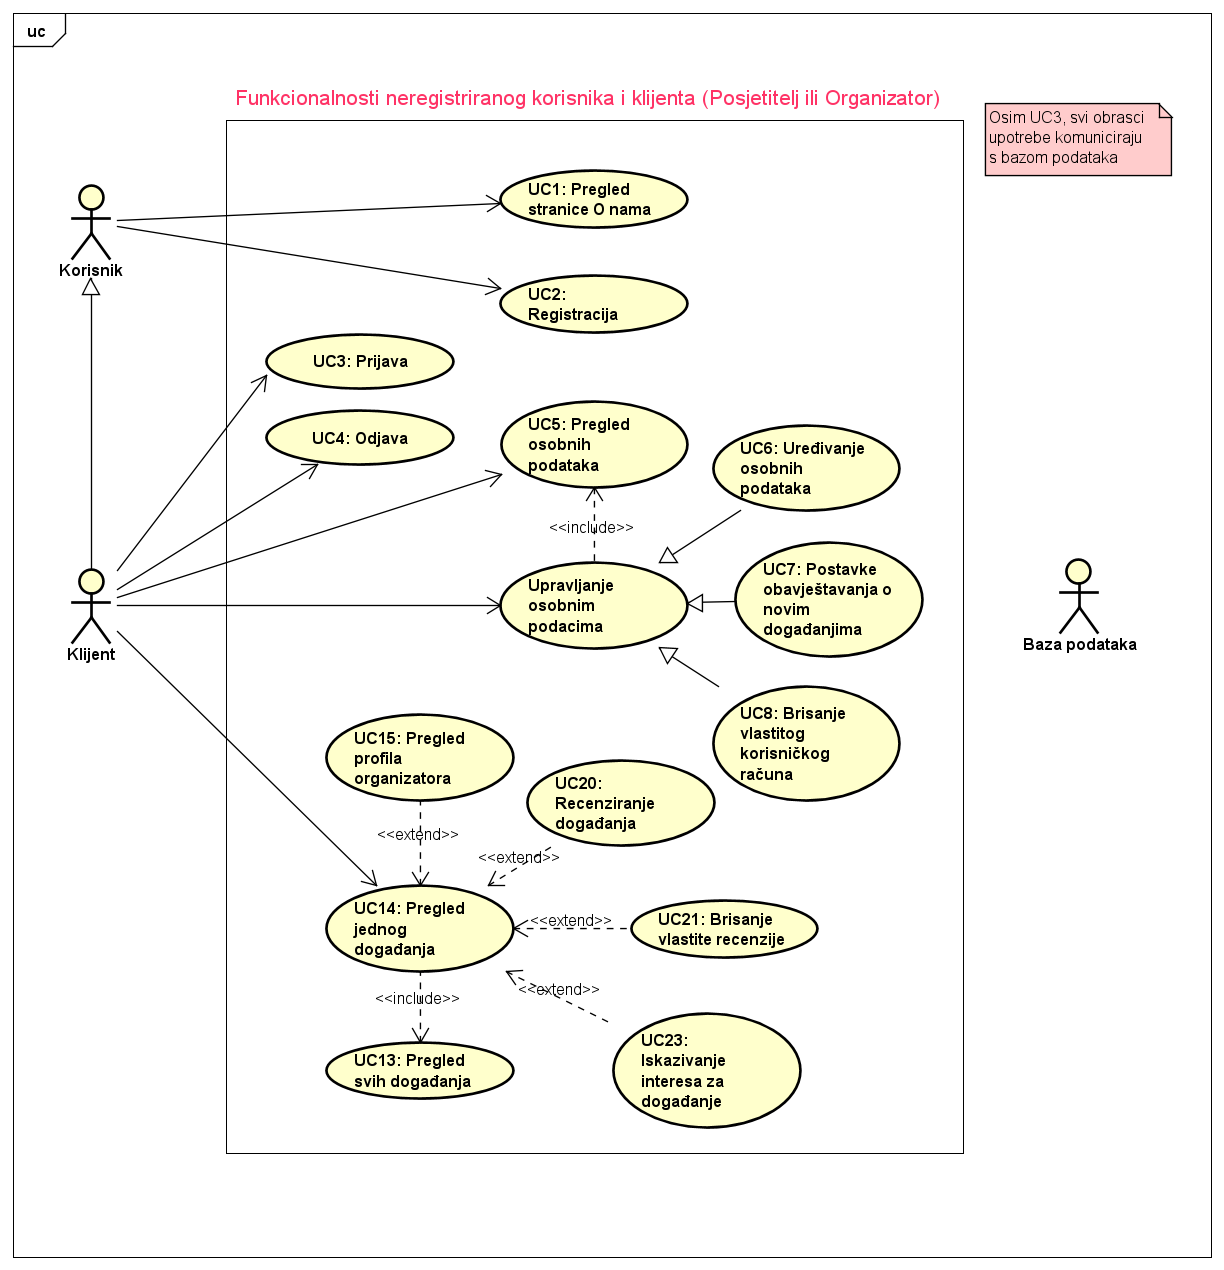
\includegraphics[scale=0.5]{dijagrami/uc1.PNG} 
					\centering
					\caption{Dijagram obrazaca uporabe, funkcionalnost Korisnika i Klijenta (Posjetitelj, Organizator)}
					\label{fig:promjene}
				\end{figure}
				
				\newpage
				
				\begin{figure}[H]
					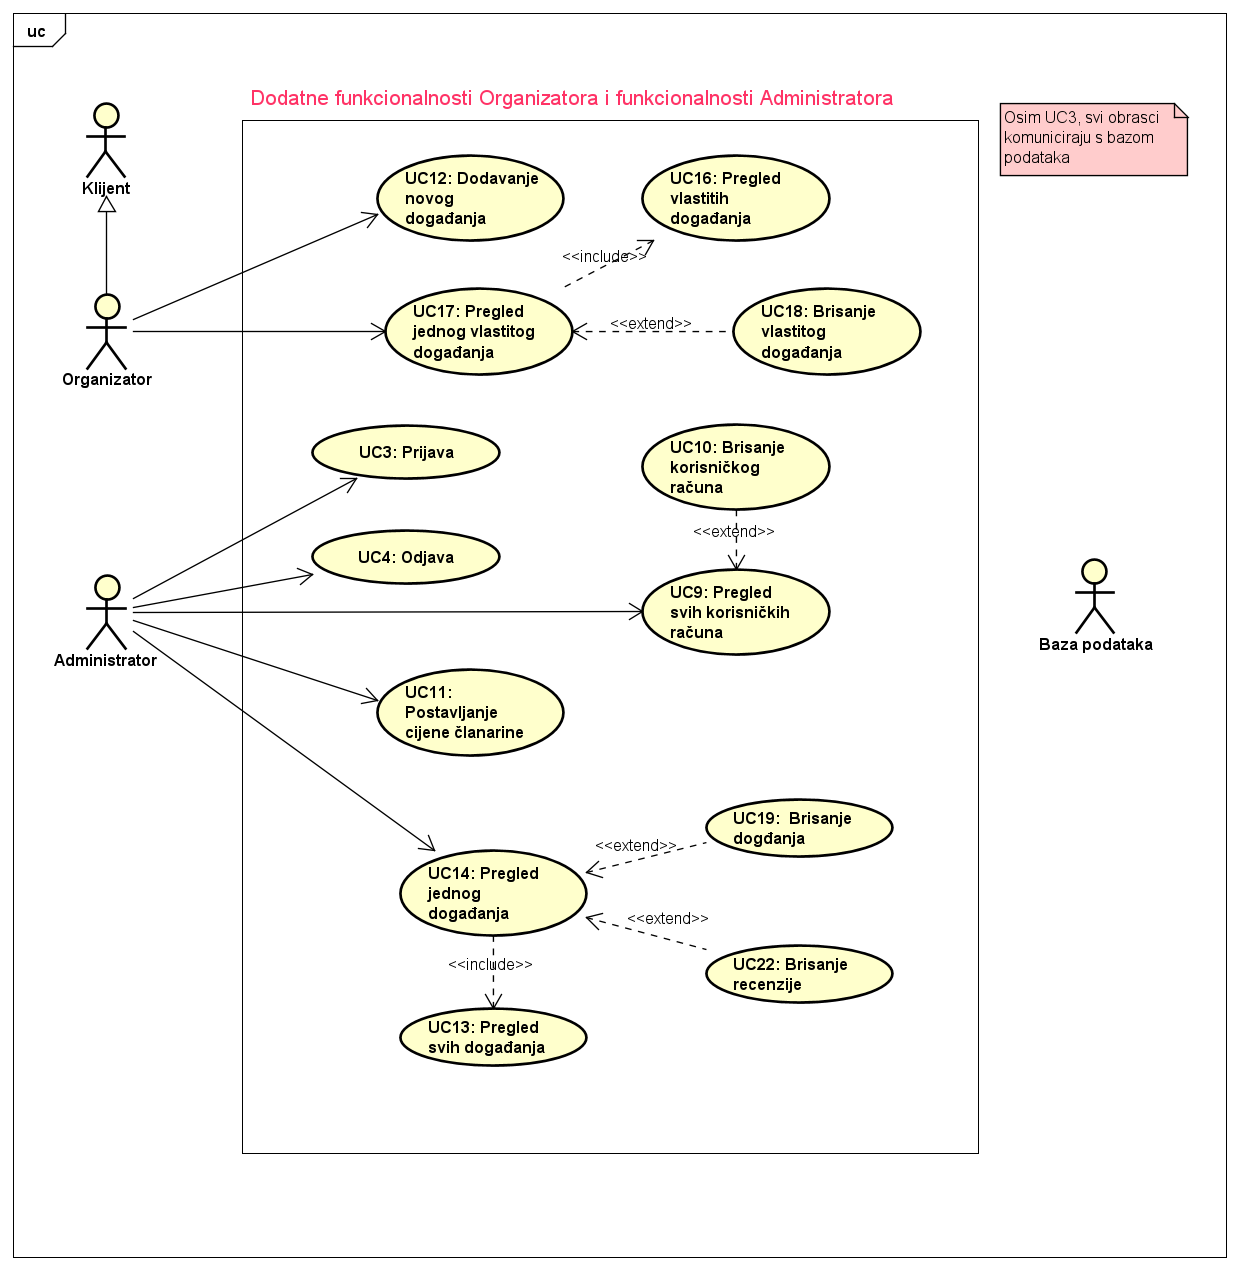
\includegraphics[scale=0.5]{dijagrami/uc2.PNG}
					\centering
					\caption{Dijagram obrazaca uporabe, dodatne funkcionalnosti Organizatora i funkcionalnost Administratora}
					\label{fig:promjene}
				\end{figure}
				
				\newpage
				
			\subsection{Sekvencijski dijagrami}
				
				\begin{figure}[H]
					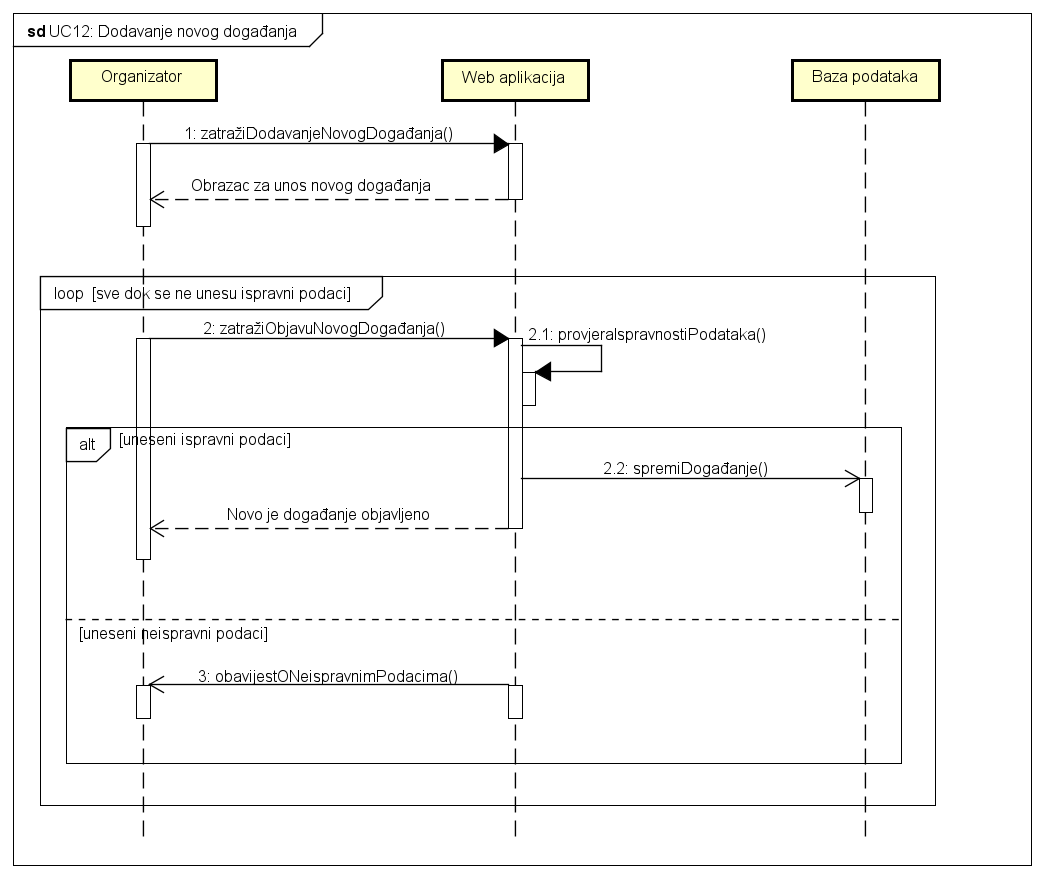
\includegraphics[width=\textwidth]{dijagrami/sd1.PNG}
					\centering
					\caption{Sekvencijski dijagram za \textbf{UC11}}
					\label{fig:promjene}
				\end{figure}
				
				\newpage
		
				
				\begin{figure}[H]
					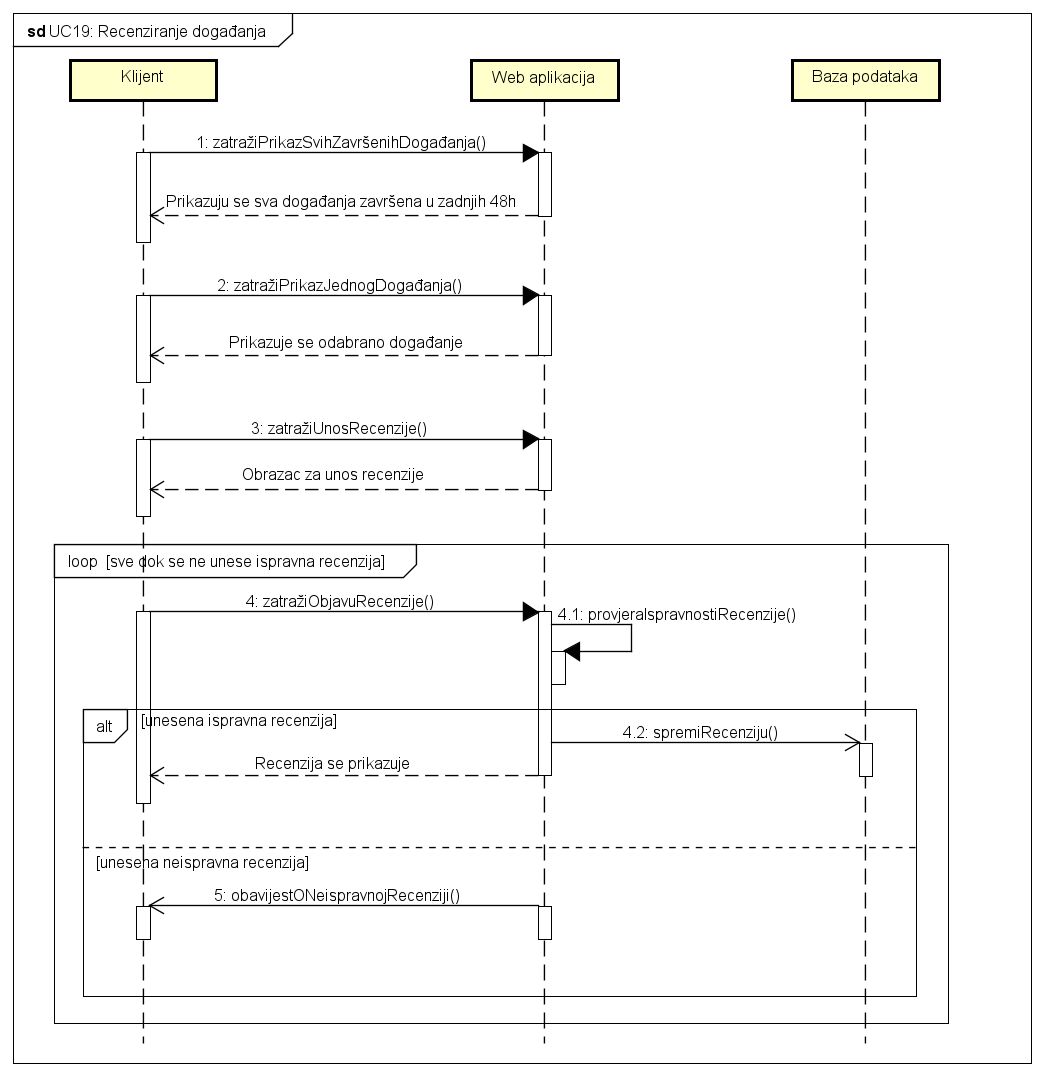
\includegraphics[width=\textwidth]{dijagrami/sd2.PNG}
					\centering
					\caption{Sekvencijski dijagram za \textbf{UC19}}
					\label{fig:promjene}
				\end{figure}
				
				\newpage
	
		\section{Ostali zahtjevi}
		
			\begin{packed_item}
				\item Sustav treba biti implementiran kao web aplikacija koristeći objektno-orijentirane jezike 
				\item Sustav mora omogućiti rad više korisnika u stvarnom vremenu 
				\item Sustav treba sve zadatke izvršavati u vrlo kratkom vremenu, unutar nekoliko sekundi
				\item Korisnički podaci trebaju biti sigurno pohranjeni i odgovarajuće enkriptirani
				\item Sustav mora efikasno pohranjivati, upravljati i pristupati podacima putem baze podataka 
				\item Korisničko sučelje mora podržavati hrvatsku abecedu pri unosu i prikazu tekstualnog sadržaja
				\item Sustav mora koristiti europsku valutu (EUR) za prikaz cijena te europski oblik datuma (\textit{DD.MM.GGGG}) za prikaz i unos datuma
				\item Web aplikacija mora biti responzivna i optimalno korisničko iskustvo pružati na svim uređajima
				\item Korisničko sučelje treba biti intuitivno i pregledno, korisnici se moraju moći koristiti sučeljem bez opširnih uputa
				\item Neispravno korištenje korisničkog sučelja ne smije narušiti funkcionalnosti i rad sustava
				
				
			\end{packed_item}
			 
			 
	